\documentclass[12pt]{article}

%%%%%%%%%%%%%%%%%%%%%%%%%%%%%%%%%%%%%%%%%%%%%%%%%%%%%%%%%%%%%%%%%%%%%%%%
%                                                                      %
%               LATEX COMMANDS FOR DOCUMENT SETUP                      %
%                                                                      %
%%%%%%%%%%%%%%%%%%%%%%%%%%%%%%%%%%%%%%%%%%%%%%%%%%%%%%%%%%%%%%%%%%%%%%%%

%\usepackage{bookmark}
\usepackage[us,nodayofweek,12hr]{datetime}
\usepackage{graphicx}

\usepackage{fullpage}
\usepackage{graphicx}
\usepackage{tabularx}
\usepackage{multirow}
\usepackage{subfigure}
\usepackage{wrapfig}
\usepackage{textcomp}
\usepackage[square, comma, numbers, sort&compress]{natbib}
\usepackage[hang,small,bf]{caption}
\usepackage{parskip}
\usepackage[margin=1in,footskip=0.5in]{geometry}
\usepackage{amsmath}
\usepackage{mdwlist}
\usepackage{epstopdf}
\usepackage[section]{placeins}

\newcommand{\para}{\vspace{5mm} \noindent}
\newcommand{\parafig}{\vspace{4mm} \noindent}
\newcommand{\paraeq}{\vspace{1mm} \noindent}
\newcommand{\negparafig}{\vspace{-4mm} \noindent}
\newcommand{\negparaeq}{\vspace{-1mm} \noindent}

\addtolength{\parskip}{1\parskip}

\bibliographystyle{plain}
%\bibliographystyle{ieeetr}
%many other bibliography styles are available (IEEEtran, mla, etc.). Use one appropriate for your field.

\hyphenation{pre-par-ing} %add hyphenation rules for words TeX doesn't know

%\usepackage[square,comma,numbers,sort&compress]{natbib}
%\usepackage{hypernat}
% Other useful packages to try
\usepackage{amsmath}
\usepackage{amssymb}
\usepackage{accents}

\usepackage{setspace}
\usepackage{algorithm}
\usepackage{algorithmic}
%
% Different fonts to try (uncomment only fontenc and one font at a time)
% (you may need to install these first)
%\usepackage[T1]{fontenc} %enable fontenc package if using one of the fonts below
%\usepackage[adobe-utopia]{mathdesign}
%\usepackage{tgschola}
%\usepackage{tgbonum}
%\usepackage{tgpagella}
%\usepackage{tgtermes}
%\usepackage{fourier}
%\usepackage{fouriernc}
%\usepackage{kmath,kerkis}
%\usepackage{kpfonts}
%\usepackage[urw-garamond]{mathdesign}
%\usepackage[bitstream-charter]{mathdesign}
%\usepackage[sc]{mathpazo}
%\usepackage{mathptmx}
%\usepackage[varg]{txfonts}


%%%%%%%%%%%%%%%%%%%%%%%%%%%%%%%%%%%%%%%%%%%%%%%%%%%%%%%%%%%%%%%%%%%%%%%%
%                                                                      %
%        DOCUMENT SETUP AND INFORMATION FOR PRELIMINARY PAGES          %
%                                                                      %
%%%%%%%%%%%%%%%%%%%%%%%%%%%%%%%%%%%%%%%%%%%%%%%%%%%%%%%%%%%%%%%%%%%%%%%%

\begin{document}

%%%%%%%%%%%%%%%%%%%%%%%%%%%%%%%%%%%%%%%%%%%%%%%%%%%%%%%%%%%%%%%%%%%%%%%%

\vspace{7cm}
\begin{center}
   {\bf\Large Mask to B-rep Paper}
\end{center}

\vspace{1.5cm}
\begin{center} 
{\bf\large Omar Hafez, Mark Rashid}\\

%\vspace{5mm}
{Department of Civil \& Environmental Engineering}\\
{University of California, Davis}\end{center}

\abstract{Abstract here}

%%%%%%%%%%%%%%%%%%%%%%%%%%%%%%%%%%%%%%%%%%%%%%%%%%%%%%%%%%%%%%%%%%%%%%%%

% Each chapter can be in its own file for easier editing and brought in with the \include command.
% Then use the \includeonly command to speed compilation when working on a particular chapter.
%%% \includeonly{chap1}

%\newcommand{\bibfont}{\singlespacing}
% need this command to keep single spacing in the bibliography when using natbib

\section{Introduction}

Image-based modeling and simulation is becoming an increasingly important analytic and predictive tool for a variety of medical and engineering applications. Some examples include patient-specific diagnosis and treatment, large-scale \textit{in silico} trials, medical device design, computer-assisted surgery, and as-built analysis of existing parts. Whereas traditional physics-based modeling and simulation typically uses NURBS-based surfaces generated from CAD software to define geometries of interest, the image-based analog extracts geometries from imaging data, typically in the form MRI or CT. The field of image-based modeling and simulation covers a broad spectrum of topics, including image processing, computational geometry, numerical methods, and continuum mechanics. The workflow entails: image acquisition, image segmentation, image-based mesh generation, and finally the application of interest. This paper focuses on one component of the image-based meshing step, namely: surface generation. The other steps are briefly mentioned below, but otherwise the focus shall remain on surface generation from a segmented image. \\ \\
%
Medical imaging is the process of generating discrete image representations of the regions of interest. For our purposes, the acquired image provides a three-dimensional rectilinear grid of point intensity values as input to the rest of the workflow. In the case of MRI, those values are weighted proton densities, which effectively measure water-content. In the case of CT, they are attenuation measurements from an x-ray beam source, which effectively measure density. For typical applications, we can expect millimeter resolution, and in some cases even better~\cite{van2012super}.\\ \\
%
Image segmentation is the process of partitioning an image into non-overlapping regions corresponding to different tissues or objects in an image. Contrast differences between neighboring tissues can be difficult to identify due in part to noise and artifacts, and thus image processing in the form of smoothing, filtering, and resampling are performed to improve the effectiveness of the image segmentation technique. The output from image segmentation consists of one or more \textit{image masks}, depending on how many regions of interest exist in the field of view. If there is only one region of interest, the output is termed a \textit{binary image mask}. A few popular techniques in image segmentation include simple thresholding, level set methods~\cite{malladi_1995, sethian_1996}, machine learning-based approaches~\cite{litjens_2017}, and often in practical cases, manual fine-tuning.\\ \\
%
Image-based meshing is the process of generating explicitly defined volume meshes from imaging data. For our purposes, we focus on generating meshes specifically from segmented image data. The challenge is to define the mesh explicitly in terms of vertex coordinates, corresponding polytopes, and the connectivity of those polytopes, as opposed to an implicit definition of the volume enclosed by the zero-set of a 4D indicator function. Image-based meshing is often separated into two steps: 1) surface generation, and 2) conventional CAD-based volume meshing. Surface generation (or surface extraction) is a matter of generating a watertight, manifold \textit{boundary representation} (or \textit{b-rep}). B-reps may refer to polygonized surface meshes or NURBS surfaces; for our purposes we will restrict the scope to surface meshes. \\ \\
%
Various approaches have been pursued to tackle image-based meshing, most of which are extensions of the \textit{marching cubes} algorithm~\cite{lorensen_1987}. It assumes an implicit isosurface exists whose associated volume is the union of voxels in an image mask that belong to the same region. Triangular patches are generated to approximate the intersection of this isosurface with each grid cell and are combined to form a continuous surface. The two most glaring limitations of the marching cubes algorithm are that 1) the resulting surfaces exhibit aliasing artifacts that poorly capture smooth and sharp features alike, and 2) the algorithm is limited to surface generation from binary masks (i.e., it cannot generate surfaces for multi-material masks). Advances in the field of image-based meshing have mostly focused on modifications to the marching cubes algorithm to address these two limitations - namely, 1) generating smooth surfaces that represent the original object accurately while preserving sharp features; and 2) generating quality surface meshes for general multi-material image masks. \\ \\ 
%
Updegrove \textit{et al.}~\cite{updegrove_2016} used a \textit{lofting} technique on a series of 2D segmentations to generate models of blood vessels. An approximate centerline must be drawn, and 2D segmentations are combined using spline interpolating functions to generate surfaces. Unstructured tetrahedral meshes are then generated from the surfaces. Lofting is known as a 2.5D approach because stacking contours of neighboring slices cannot capture arbitrary 3D topologies. The approach often suffers from significant loss of accuracy, and the interpolating splines typically require manual selection of control points~\cite{young_2008}. Treating an image mask as a series of 2D masks was a popular approach in past decades, but most modern approaches treat it as a three-dimensional object to avoid the drawbacks of lofting techniques. \\ \\
%
Young \textit{et al.}~\cite{young_2008} used a \textit{direct meshing} approach to generate meshes from multi-material image masks without the intermediate step of creating a surface mesh. Young \textit{et al.} combined the surface generation and mesh generation stages into one process via their \textit{enhanced volumetric marching cubes} approach. Standard volumetric marching cubes generates tetrahedral volumes from the intersection of the isosurface with grid cells, rather than just triangular surface patches. The authors extended the volumetric algorithm to handle intersections of up to eight regions in one grid cell - the maximum number of intersections that can occur for a Cartesian grid. The resulting mesh is \textit{mixed hex-tet}, where tetrahedra exist near the surface based on the extended volumetric marching cubes approach; internal voxels are converted directly to hexahedra; and pyramidal and tetrahedral elements exist in the transitional layer in between. The authors also utilized partial volume-based interpolation to improve surface smoothness. Additional efforts to reduce the mesh size were made by converting surface tetrahedra to hexahedra where appropriate, and by performing an octree-based approach to collect neighboring interior hexahedral elements into larger elements. Nonetheless, this \textit{grid-based} approach results in a surface mesh that is very fine, which subsequently constrains the size of interior elements in the volume mesh. The resulting mesh from this approach yields an intractably large number of degrees of freedom for simulation purposes. Thus, for practical purposes, the number of points and polyhedra defining the surface must be reduced (or \textit{decimated}), to allow for a subsequent coarser volumetric discretization. Indeed, the default and recommended approach in their software \textit{Simpleware} (known as \textit{+FE Free}) is to follow the two-step paradigm of surface generation followed by CAD-based meshing as described previously. Namely, the software extracts the resulting surface following the extended volumetric marching cubes step, performs multi-part decimation and smoothing~\cite{egst}, and finally uses a conventional CAD-based tetrahedral mesher to generate fully tetrahedral meshes from the polygonized surfaces. \\ \\
%
Meyer \textit{et al.}~\cite{meyer_2008} employed a \textit{particle-based sampling} technique for multi-material volumes. Surface samples (called \textit{particles}) are constrained to the zero-set of an implicit function. The distances between particles are locally adapted to create higher densities of points near surface features. A Delaunay tetrahedralization of the sampling points is computed, and each tetrahedron is assigned a material label. The surface mesh is generated by extracting the faces bounded by tetrahedra with different material labels. Finally, a conventional CAD-based tetrahedral mesher is once again employed to produce an analysis-ready mesh. The approach faithfully and robustly captures the geometries of complex material interfaces, but has debilitating performance issues, even by the own admission of the authors. \\ \\
%
A number of other techniques have been published on the topic of image-based meshing, often attacking the problem from completely different perspectives~\cite{fang_2009, mohamed_2004, jermyn_2013, boissonnat_2009}. Although several of the works presented here attempt to generate surfaces for multi-material image masks, a great deal of effort and applicability still exists for generating high-quality surfaces (and resulting meshes) from binary image masks. This will be the focus of the paper, as we propose a novel Voronoi-based surface generation approach that guarantees watertightness and lays out a framework that has the potential to ultimately reconstruct a wider array of boundaries, including those with sharp edges or corners. The method is also simple to use, freeing the user from a complicated set of parameters that need to be modified for optimal results. \\ \\
%
Provided a triangulated surface mesh from any of the aforementioned approaches, conventional CAD-based volume-meshing techniques are utilized to produce a final volume mesh. Since a general automatic hexahedral meshing algorithm has yet to be developed, tetrahedral meshing is usually the method of choice for arbitrary input surfaces. The two most widely adopted approaches for automated unstructured tetrahedral mesh generation are \textit{advancing front}~\cite{jin_1993, lohner_1988} and \textit{Delaunay tetrahedralization}~\cite{lohner_1997}. \\ \\
%
Finally, applications for this work range from 3D printing to visualization to finite element analysis (FEA). In the case of 3D printing and visualization, b-reps can be used for surgery planning, custom surgical guides and implants, rapid prototyping, and generation of CAD surfaces from existing parts. Meanwhile, image-based simulation has been performed on nearly every major organ in the body and shows great promise in advancing both personalized medicine~\cite{neal2010current} and large-scale clinical trials~\cite{viceconti2016silico}. In addition, image-based simulation offers the ability to perform non-destructive analysis on as-built engineering parts or legacy parts whose CAD may not be available~\cite{bradley2005advances}.\\ \\
%
Given the context of the image-based modeling and simulation workflow within which it fits, the novel Voronoi-based surface generation method is now proposed herein. The algorithm is followed by a performance assessment in comparison to a state-of-the-art commercial software, which are made for a variety of canonical cases as well as for cases from real MRI and CT data. The paper is closed with a summary and discussion of future directions for this work.

\section{Incremental Kinematics}
%

\newcommand{\ds}{\displaystyle}
\newcommand{\mparen}[1]{\displaystyle \big( #1 \big)}
\newcommand{\mbrack}[1]{\displaystyle \big[ #1 \big]}
\newcommand{\bparen}[1]{\displaystyle \bigg( #1 \bigg)}
\newcommand{\bbrack}[1]{\displaystyle \bigg[ #1 \bigg]}

The Jaumann rate of stress for a linear hypoelastic material is characterized by:

$$ \overset{\Delta}{\sigma} \equiv 
\dot{\sigma} + \sigma \cdot W - W \cdot \sigma = 
C : D $$

where $ D = \frac{1}{2} (L + L^\top), \; W = \frac{1}{2} (L - L^\top)$, and $L = \dot{F}
F^{-1} $. We would like to know how the stress state changes after applying
a prescribed deformation. Our approach is as follows: parameterize the deformation
into separate stages of pure stretch and pure rotation. The advantage of this
approach is that it allows the terms in the stress rate above to be integrated
separately

\begin{align*}
\dot{\sigma} = 
\begin{cases}
C : D & \qquad \text{W vanishes for pure stretch} \\
W \cdot \sigma - \sigma \cdot W & \qquad \text{D vanishes for pure rotation}
\end{cases}
\end{align*}

Simple analytic solutions exist for each of these ordinary differential equations, 
provided that $D, W$ are constant ($C$ is also assumed to be constant):

\begin{align*}
\dot{\sigma}(t) = C : D, \; \sigma(0) = \sigma_i 
\qquad 
& \Longrightarrow 
\qquad 
\sigma_{i+\frac{1}{2}}  = \sigma_i + C : D \Delta t \\ \\
\dot{\sigma}(t) = W \cdot \sigma - \sigma \cdot W, \; \sigma(0) = \sigma_{i+\frac{1}{2}} 
\qquad 
& \Longrightarrow 
\qquad 
\sigma_{i+1} = \exp(W \Delta t) \; \sigma_{i+\frac{1}{2}} \; \exp(W \Delta t)^{\top}
\end{align*}

Combining these two results gives us our stress update procedure:

$$ \sigma_{i+1} = \exp(W \Delta t) \; \bparen{\sigma_i + C : D \Delta t} \; \exp(W \Delta t)^{\top} $$

All that remains is to find reasonable approximations for $D, W$. To that end, we
consider the polar decomposition of the incremental deformation gradient, 
$F = R \; U$. After taking a time derivative of $F$, and substituting into the
definition of $L$, we get:

$$ L \equiv D + W = \dot{R} \; R^\top + R \; \dot{U} \; U^{-1} \; R^\top $$

When considering the separate stages of pure stretch and pure rotation, this
equation reduces to:

\begin{align*}
\begin{cases}
D = \dot{U} \; U^{-1} & \qquad \text{pure stretch} \\
W = \dot{R} \; R^\top & \qquad \text{pure rotation}
\end{cases}
\end{align*}

These are constant-coefficient, ordinary differential equations
than can be used to determine $D$ and $W$. The
general solution for equations of this form is

$$ 
Y = \dot{X} X^{-1}, \; X(0) = \mathbf{1} 
\qquad 
\Longrightarrow 
\qquad 
X(\Delta t) = \exp(Y \Delta t)
$$

Which, when applied to the pure stretch and pure rotation versions of the problem
gives us our definitions of $D, W$:

$$ D = \frac{1}{\Delta t} \log(U), \qquad W = \frac{1}{\Delta t} \log(R) $$

Substituting these back into our stress update procedure gives 

$$\boxed{\sigma_{i+1} = R \; \bparen{\sigma_i + C : \log(U)} \; R^\top}$$




%%%%%%%%%%%%%%%%%%%%%%%%%%%%%%%%%%%%%%%%%%%%%%%
%%%%%%%%%%%%%%%%%%%%%%%%%%%%%%%%%%%%%%%%%%%%%%%
\subsection{Description}
\label{Description}

%%%%%%%%%%%%%%%%%%%%%%%%%%%%%%%%%%%%%%%%%%%%%%%
%%%%%%%%%%%%%%%%%%%%%%%%%%%%%%%%%%%%%%%%%%%%%%%
\subsection{Implementation Approaches}
\label{Implementation Approaches}
%%%%%%%%%%%%%%%%%%%%%%%%%%%%%%%%%%%%%%%%%%%%%%%
%%%%%%%%%%%%%%%%%%%%%%%%%%%%%%%%%%%%%%%%%%%%%%%
\subsubsection{Hughes-Winget}
\label{Hughes-Winget}

\subsubsection{Rashid}
\label{Rashid}

hi
\section{Finite Element Residual and Tangent Stiffness}
%

This section discusses the greater context of solid mechanics, and the corresponding finite element system of equations in the presence of finite deformations. According to the developments of the previous section, a strongly objective kinematic algorithm and its implementation are proposed in this setting.

For a continuum body which occupies an open domain $\Omega_0 \subset \mathbb{R}^d$ in its undeformed configuration, the weak form equations of equilibrium may be expressed as
\begin{equation}
    R_{i} \equiv \int_{\Omega_0} P_{ij} \phi_{,j} \, d \Omega_0 + \int_{\Gamma_0} p_i \phi \, d \Gamma_0 = 0 \quad \forall i, \phi \in H^1_0 (\Omega_0),
\end{equation}
where $\mathbf{P}$ represents the first Piola-Kirchhoff stress tensor, and $\mathbf{p}$ is the Piola traction vector. This representation is amenable to a total Lagrangian approach.

Discuss the need for a consistent linearization of the residual for use in a non-linear Newton solver.

Perhaps without even referring to finite elements, discuss the computations that are needed at the quadrature-point level.

Explain the steps needed for the evaluation of the residual contribution (at a quadrature point), and correspondingly for the evaluation of the tangent contribution:

Elaborate on how to compute exact derivatives of the relevant quantities

include all the derivatives\\
a complete, full implementation, with code snippet\\
potentially Sam working on an improved (more novel) implementation of what Mark did\\

\subsection{Generalized Material Update}

In a continuum body $\Omega_0$, a given material point $\mathbf{X} \in \Omega_0$ is endowed with a ``material state'' $S_k (\mathbf{X})$ at time $t_k$. In the context of Lagrangian solid mechanics, the material state $S_k = \left\{ \boldsymbol{\sigma}_{k}, \, q_{*k} \right\}$ consists of the Cauchy stress tensor $\boldsymbol{\sigma}_{k}$, and any (possibly tensorial) internal state variables $q_{*k}$ associated with the material model.

According to the Lagrangian description of motion, a material point initially located at a position $\mathbf{X} \in \Omega_0$ will occupy the spatial position $\mathbf{x}_k$ at some later time $t_k$, undergoing a total displacement $\mathbf{u}_k = \mathbf{x}_k - \mathbf{X}$. In a computational setting, the analysis is subdivided into discrete time steps $\left\{ t_k \right\}_{k=0}^N$, and the motion of material points from time $t_k$ to $t_{k+1}$ is described by an incremental displacement field, denoted $\hat{\mathbf{u}} = \mathbf{u}_{k+1} - \mathbf{u}_{k}$. The deformation associated with this motion may be characterized by an incremental deformation gradient $\hat{\mathbf{F}} = \partial \mathbf{x}_{k+1} / \partial \mathbf{x}_k = \mathbf{1} + \nabla \hat{\mathbf{u}}$. This representation of the deformation taking place in discrete increments is equally suitable for updated or total Lagrangian formulations.

Assuming that the material behaves in a rate-independent manner, a generic material update procedure $f \colon (S_k, \nabla \hat{\mathbf{u}}) \mapsto S_{k+1}$ should yield the updated material state $S_{k+1}$ at time $t_{k+1}$ as a function of the material state $S_k$ at time $t_k$, and the incremental displacement gradient $\nabla \hat{\mathbf{u}}$. The updated stress may then be used to evaluate residual force contributions. If a tangent stiffness matrix must be constructed, the material update procedure must also evaluate the tangent derivatives of the Cauchy stress with respect to the input deformation (i.e. $\partial \boldsymbol{\sigma}_{k+1} / \partial \nabla \hat{\mathbf{u}}$).

Within this generalized framework, the displacement gradient may be optionally modified prior to being passed into the material update procedure, in such a fashion as to accommodate mixed or enhanced degrees of freedom (should these be present), or to apply a strain projection methodology (e.g. an F-bar approach).

\subsection{Hypoelastic Material Update}

For a hypoelastic material, the constitutive model is expressed in rate form:
\begin{equation}
        \accentset{\circ}{\boldsymbol{\sigma}} = \mathbb{C} : \mathbf{D},
\end{equation}
where $\accentset{\circ}{\boldsymbol{\sigma}}$ denotes a particular co-rotational rate of the Cauchy stress (e.g. the Jaumann stress rate), and $\mathbb{C}$ depends upon the material state.

Most numerical implementations for rate-independent material models of this type consider an increment of strain $\Delta \boldsymbol{\varepsilon}$ as the driving input variable, which is used to evolve the material state via a constitutive update procedure (denoted as $C$), such that
\begin{equation}
    S_{k+1} = C (S_{k}, \Delta \boldsymbol{\varepsilon}).
\end{equation}
Additionally, a tangent material modulus $\partial \boldsymbol{\sigma}_{k+1} / \partial \Delta \boldsymbol{\varepsilon}$ may be requested if stiffness contributions are needed.

The foregoing constitutive update procedure is sufficient for problems involving small deformations. In the presence of finite deformations, however, an additional procedure $R$ must be defined to allow for rotation of the material state, i.e.
\begin{equation}
    S_{k+1} = R (S_k, \mathbf{R}),
\end{equation}
such that $\boldsymbol{\sigma}_{k+1} = \mathbf{R} \boldsymbol{\sigma}_{k} \mathbf{R}^T$, and where the material's internal state variables $q_{*k}$ are rotated according to their tensorial character (e.g. $\mathbf{q}_{k+1} = \mathbf{R} \mathbf{q}_k$ if $\mathbf{q}_k$ is a vector-valued quantity). If an evaluation of stiffness terms is required, $\partial \boldsymbol{\sigma}_{k+1} / \partial \mathbf{R}$ must be computed, as well.

Given an input deformation $\nabla \hat{\mathbf{u}}$, it is therefore of interest to compute corresponding strain and rotation increments ($\Delta \boldsymbol{\varepsilon}$ and $\hat{\mathbf{R}}$, respectively) which may be used to update the material state in a step-wise sequence via
\begin{equation}
    S_{k+1} = R\big(C(S_k, \Delta \boldsymbol{\varepsilon}), \hat{\mathbf{R}}\big),
\end{equation}
or alternatively,
\begin{equation}
    S_{k+1} = C\big(R(S_k, \hat{\mathbf{R}}), \Delta \boldsymbol{\varepsilon}\big).
\end{equation}
This necessitates the specification of a ``kinematic splitting'' algorithm $K$ of the form
\begin{equation}
    \left\{ \Delta \boldsymbol{\varepsilon}, \, \hat{\mathbf{R}} \right\} = K(\nabla \hat{\mathbf{u}}),
\end{equation}
which should also be capable of supplying kinematic tangent terms (i.e. $\partial \Delta \boldsymbol{\varepsilon} / \partial \nabla \hat{\mathbf{u}}$ and $\partial \hat{\mathbf{R}} / \partial \nabla \hat{\mathbf{u}}$).

Given a set $\left\{ K, C, R \right\}$ consisting of the aforementioned procedures, a generic hypoelastic meterial update is formulated in algorithm \ref{alg:hypoelastic_update} which is valid for rate independent models.
\begin{algorithm}
\begin{spacing}{1.3}
 \caption{Hypoelastic material update procedure for rate independent models}
 \label{alg:hypoelastic_update}
 \begin{algorithmic}[1]
 \renewcommand{\algorithmicrequire}{\textbf{Input:  }}
 \renewcommand{\algorithmicensure}{\textbf{Output:  }}
 \REQUIRE $S_k$ and $\nabla \hat{\mathbf{u}}$
 \ENSURE  $S_{k+1}$ (optionally $\partial \boldsymbol{\sigma}_{k+1} / \partial \nabla \hat{\mathbf{u}}$)
    \\ \textit{Kinematic split} :
    \STATE $\left\{ \Delta \boldsymbol{\varepsilon}, \, \hat{\mathbf{R}} \right\} = K(\nabla \hat{\mathbf{u}})$ (optionally compute $\partial \Delta \boldsymbol{\varepsilon} / \partial \nabla \hat{\mathbf{u}}$ and $\partial \hat{\mathbf{R}} / \partial \nabla \hat{\mathbf{u}}$)
    \\ \textit{Constitutive update} :
    \STATE $S_{k+\frac{1}{2}} = C (S_k, \, \Delta \boldsymbol{\varepsilon})$ (optionally compute $\partial \boldsymbol{\sigma}_{k+\frac{1}{2}} / \partial \Delta \boldsymbol{\varepsilon}$)
    \\ \textit{Rotate state} :
    \STATE $S_{k+1} = R (S_{k+\frac{1}{2}}, \hat{\mathbf{R}})$ (optionally compute $\partial \boldsymbol{\sigma}_{k+1} / \partial \hat{\mathbf{R}}$)
    \\ \textit{(Optionally) compute an algorithmically consistent tangent} :
    \STATE $\frac{\partial \boldsymbol{\sigma}_{k+1}}{\partial \nabla \hat{\mathbf{u}}} = \frac{\partial \boldsymbol{\sigma}_{k+1}}{\partial \hat{\mathbf{R}}} : \frac{\partial \hat{\mathbf{R}}}{\partial \nabla \hat{\mathbf{u}}} + R \big(\frac{\partial \boldsymbol{\sigma}_{k+1/2}}{\partial \Delta \boldsymbol{\varepsilon}} : \frac{\partial \Delta \boldsymbol{\varepsilon}}{\partial \nabla \hat{\mathbf{u}}}, \hat{\mathbf{R}}\big)$
 \end{algorithmic}
 \end{spacing}
 \end{algorithm}
 
\subsection{Kinematic Splitting Algorithm}

The specification of an appropriate kinematic splitting algorithm depends on two primary considerations: the objective stress rate with which the intended algorithm is to maintain consistency, and the desired level of accuracy that the algorithm should achieve.

A material update procedure is called \textit{consistent} with a given objective stress rate if the truncation error $\tau(\Delta t)$ of the algorithm approaches zero in the limit as $\Delta t \rightarrow 0$, i.e.
\begin{equation}
    \lim_{\Delta t \rightarrow 0} \tau (\Delta t) = 0.
\end{equation}
It suffices to show that 
\begin{equation}
    \lim_{\Delta t \rightarrow 0} \frac{\boldsymbol{\sigma}_{k+1} - \boldsymbol{\sigma}_{k}}{\Delta t} = \accentset{\circ}{\boldsymbol{\sigma}} + \mathbf{W} \cdot \boldsymbol{\sigma} - \boldsymbol{\sigma} \cdot \mathbf{W},
\end{equation}
where $\Delta t = t_{k+1} - t_{k}$. It can be easily shown that algorithm \ref{alg:hypoelastic_update} is consistent with the Jaumann rate, provided an appropriate kinematic splitting algorithm is employed.


\begin{algorithm}
\begin{spacing}{1.2}
 \caption{Strongly objective kinematic splitting algorithm}
 \label{alg:kinematic_splitting}
 \begin{algorithmic}[1]
 \renewcommand{\algorithmicrequire}{\textbf{Input:  }}
 \renewcommand{\algorithmicensure}{\textbf{Output:  }}
 \REQUIRE $\nabla \hat{\mathbf{u}}$
 \ENSURE $\Delta \boldsymbol{\varepsilon}$ and $\hat{\mathbf{R}}$ (optionally $\partial \Delta \boldsymbol{\varepsilon} / \partial \nabla \hat{\mathbf{u}}$ and $\partial \hat{\mathbf{R}} / \partial \nabla \hat{\mathbf{u}}$)
    \\ \textit{Compute the incremental Green-Lagrange strain} :
    \STATE $\hat{\mathbf{E}} = \frac{1}{2}(\hat{\mathbf{C}} - \mathbf{1}) = \frac{1}{2}(\nabla \hat{\mathbf{u}} + \nabla \hat{\mathbf{u}}^T + \nabla \hat{\mathbf{u}}^T \nabla \hat{\mathbf{u}})$
    \\ \textit{Compute the eigendecomposition} :
    \STATE $\frac{1}{2} \mathbf{Q} (\boldsymbol{\Lambda}^2 - \mathbf{1}) \mathbf{Q}^T = \text{eig} (\hat{\mathbf{E}})$
    \\ \textit{Compute the rotation increment} :
    \STATE $\hat{\mathbf{R}} = (\mathbf{1} + \hat{\mathbf{u}}) \mathbf{Q} \boldsymbol{\Lambda}^{-1} \mathbf{Q}^T$
    \\ \textit{Compute the logarithmic strain increment} :
    \STATE $\Delta \boldsymbol{\varepsilon} = \mathbf{Q} \log (\boldsymbol{\Lambda}) \mathbf{Q}^T$
 \end{algorithmic}
 \end{spacing}
 \end{algorithm}


\section{Examination of Numerical Accuracy}


%%%%%%%%%%%%%%%%%%%%%%%%%%%%%%%%%%%%%%%%%%%%%%%
%%%%%%%%%%%%%%%%%%%%%%%%%%%%%%%%%%%%%%%%%%%%%%%
\FloatBarrier
\subsection{Uniaxial Compression with Finite Rotation}
%
For the sake of comparison with the strongly objective algorithm proposed in \cite{rashid1993}, an example problem similar to the one given therein will be considered, consisting of a block of isotropic material which is compressed uniaxially and simultaneously rotated according to the deformation gradient given by
\begin{equation}
    \mathbf{F} = \mathbf{R} \mathbf{U} = \left[ \begin{array}{ccc} \cos \omega t & - \sin \omega t & 0 \\ \sin \omega t & \cos \omega t & 0 \\ 0 & 0 & 1 \end{array} \right] \left[ \begin{array}{ccc} 1 - \beta t & 0 & 0 \\ 0 & 1 & 0 \\ 0 & 0 & 1 \end{array} \right],
\end{equation}
The material model will be chosen as the isotropic hypoelastic model of grade zero, i.e.
\begin{equation}
    \overset{\circ}{\mathbf{T}} = \lambda \mathbf{1} \text{tr} (\mathbf{D}) + 2 \mu \mathbf{D},
\end{equation}
where $\lambda = E \nu / (1+\nu)(1-2\nu)$ and $\mu = E/2(1+\nu)$ are the standard Lam\'{e} parameters. Exact solutions for the Cauchy stress components according to the Jaumann rate are easily obtained for this problem:
\begin{equation}
  \left\{ \begin{array}{c} T_{11} \\ T_{22} \\ T_{33} \\ T_{23} \\ T_{13} \\ T_{12} \end{array} \right\} = \left\{ \begin{array}{c} \left[ \lambda + \mu (1 - \cos 2 \omega t) \right] \ln (1 - \beta t) \\ \left[ \lambda + \mu (1 + \cos 2 \omega t) \right] \ln (1-\beta t) \\ \lambda \ln (1-\beta t) \\ 0 \\ 0 \\ -\mu (\sin 2 \omega t) \ln (1-\beta t) \end{array} \right\}.
\end{equation}
Numerical solutions were computed for the values $\omega = \pi$, $\beta = 0.5$, $E = 2.09 \times 10^5$, $\nu = 0.3$, and $t \in \left[ 0, 1 \right]$. The results are depicted in figure \ref{fig.v1-cm1}.

\begin{figure}
\centering
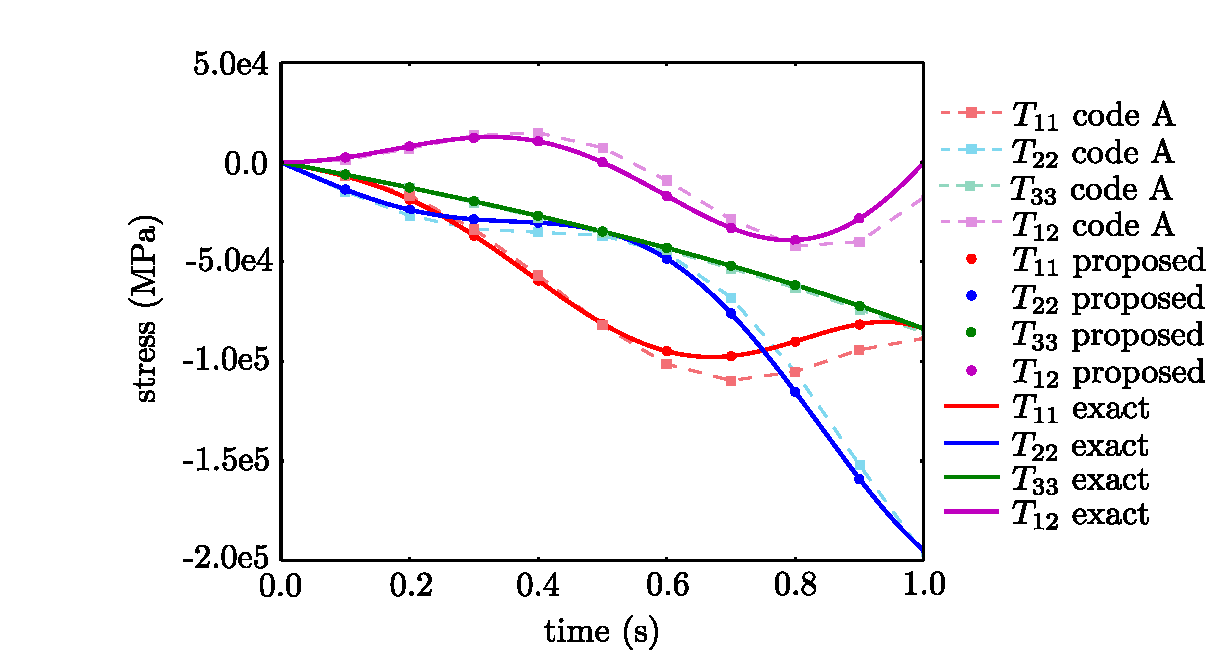
\includegraphics[scale=0.75]{media/stretch_rotate.pdf}
% where an .eps filename suffix will be assumed under latex,
% and a .pdf suffix will be assumed for pdflatex
\caption{Stress components plotted vs. time for the problem of uniaxial compression with finite rotation.}
\label{fig.v1-cm1}
\end{figure}

Worst-case relative errors between the exact solution $\mathbf{T}$ and approximate solutions $\mathbf{T}^h$ were computed via
\begin{equation}
    \text{\% error } (\mathbf{T}^h) = \sqrt{\frac{\max_{t} (\mathbf{T}^h - \mathbf{T}) \colon (\mathbf{T}^h - \mathbf{T})}{\max_{t} \mathbf{T} \colon \mathbf{T}}} \times 100 \% ,
    \label{eq:relative_error}
\end{equation}
and tabulated in table \ref{tab.v1-cm1}.

\begin{table}[]
\centering
\caption{Relative errors for the problem of uniaxial compression with finite rotation}
\label{tab.v1-cm1}
\begin{tabular}{c|c|c|c}
& code A & Rashid (1993) & proposed algorithm  \\ \hline
\% error $(\mathbf{T}^h)$ & 11.21704 & 0.01718 & 0.00014
\end{tabular}
\end{table}

%%%%%%%%%%%%%%%%%%%%%%%%%%%%%%%%%%%%%%%%%%%%%%%
%%%%%%%%%%%%%%%%%%%%%%%%%%%%%%%%%%%%%%%%%%%%%%%
\FloatBarrier
\subsection{Cyclic Shear}
%
In a retrospective examination of solution accuracy, the problem discussed in \cite{rashid1996} will be examined within the present context. The problem consists of a block of material which is subjected to a simple, cyclic shearing deformation given by
\begin{equation}
    \mathbf{F} = \left[ \begin{array}{ccc} 1 & \gamma & 0 \\ 0 & 1 & 0 \\ 0 & 0 & 1 \end{array} \right], \qquad \mathbf{L} = \left[ \begin{array}{ccc} 0 & \dot{\gamma} & 0 \\ 0 & 0 & 0 \\ 0 & 0 & 0 \end{array} \right],
\end{equation}
and where
\begin{equation}
    \gamma (t) = 2 \Gamma \bigg( \frac{2t}{T} - \left\lfloor \frac{2t}{T} + \frac{1}{2} \right\rfloor \bigg) (-1)^{\left\lfloor \frac{2t}{T} + \frac{1}{2} \right\rfloor}
\end{equation}
corresponds to the triangle wave with period $T$ and peak amplitude $\Gamma$, whose time derivative
\begin{equation}
    \dot{\gamma} (t) = \frac{4 \Gamma}{T} (-1)^{\left\lfloor \frac{2t}{T} + \frac{1}{2} \right\rfloor}
\end{equation}
is the square wave with period $T$. As before, the isotropic hypoelastic model of grade zero will be employed, where $\mu = E/2(1+\nu)$ represents the shear modulus of the material. The exact solution for the Cauchy stress components according to the Jaumann rate is given by the solution to the differential equation:
\begin{equation}
    \left\{ \begin{array}{c} \dot{T}_{11} \\ \dot{T}_{22} \\ \dot{T}_{12} \end{array} \right\} = \left[ \begin{array}{ccc} 0 & 0 & \dot{\gamma} \\ 0 & 0 & - \dot{\gamma} \\ -\dot{\gamma}/2 & \dot{\gamma}/2 & 0 \end{array} \right] \left\{ \begin{array}{c} T_{11} \\ T_{22} \\ T_{12} \end{array} \right\} + \mu \left\{ \begin{array}{c} 0 \\ 0 \\ \dot{\gamma} \end{array} \right\},
\end{equation}
which yields
\begin{equation}
    \left\{ \begin{array}{c} T_{11} \\ T_{22} \\ T_{33} \\ T_{23} \\ T_{13} \\ T_{12} \end{array} \right\} = \left\{ \begin{array}{c} \mu (1-\cos \gamma (t)) \\ \mu (\cos \gamma (t) - 1) \\ 0 \\ 0 \\ 0 \\ \mu \sin \gamma (t) \end{array} \right\}.
\end{equation}
Numerical solutions were computed for the values $\Gamma = 0.5$, $E = 2.09 \times 10^5$, $\nu = 0.3$, $T = 1.0$, and $t \in \left[ 0, 2 \right]$, yielding 2 complete cycles of deformation. The results are depicted in figure \ref{fig.cyclic_shear-cm1}.

\begin{figure}
\centering
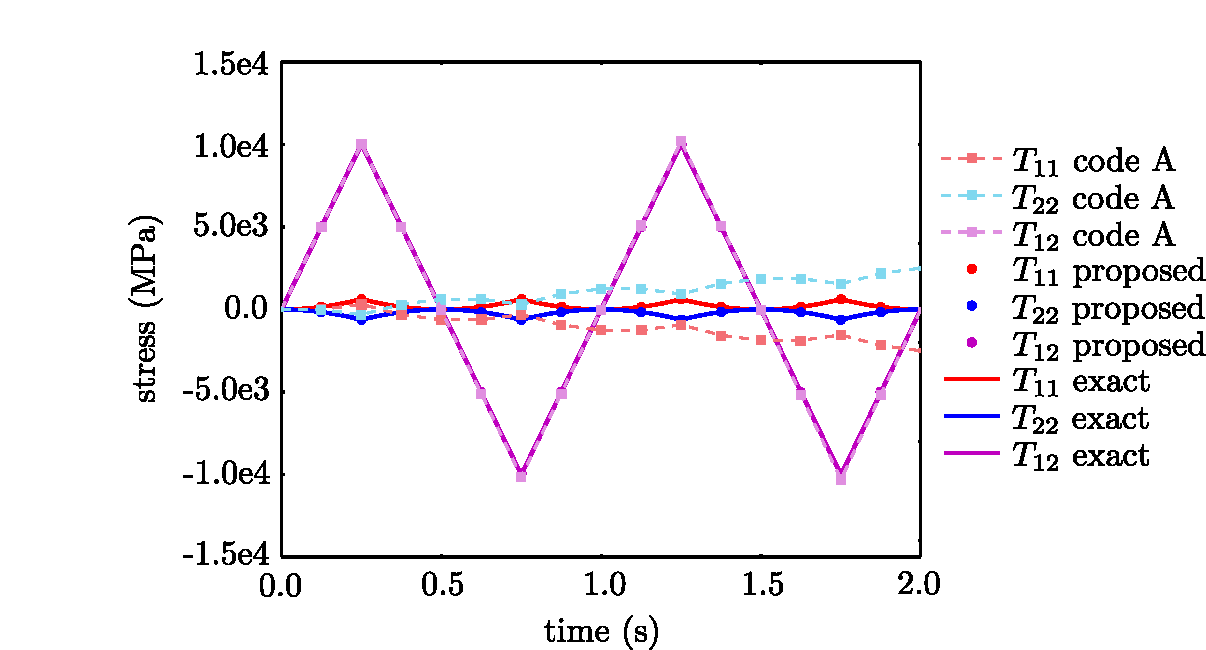
\includegraphics[scale=0.75]{media/cyclic_shear.pdf}
% where an .eps filename suffix will be assumed under latex,
% and a .pdf suffix will be assumed for pdflatex
\caption{Stress components plotted vs. time for the problem of cyclic shear.}
\label{fig.cyclic_shear-cm1}
\end{figure}

Worst-case relative errors between the exact solution $\mathbf{T}$ and approximate solutions $\mathbf{T}^h$ were computed via equation \ref{eq:relative_error} and tabulated in table \ref{tab.cyclic_shear-cm1}.

\begin{table}[]
\centering
\caption{Relative errors for the problem of cyclic shear}
\label{tab.cyclic_shear-cm1}
\begin{tabular}{c|c|c|c}
& code A & Rashid (1993) & proposed algorithm  \\ \hline
\% error $(\mathbf{T}^h)$ & 24.94638 & 0.00227 & 0.00205
\end{tabular}
\end{table}

%%%%%%%%%%%%%%%%%%%%%%%%%%%%%%%%%%%%%%%%%%%%%%%
%%%%%%%%%%%%%%%%%%%%%%%%%%%%%%%%%%%%%%%%%%%%%%%
\FloatBarrier
\subsection{Twisting Prism}

\begin{figure}[!tbhp]
\centering
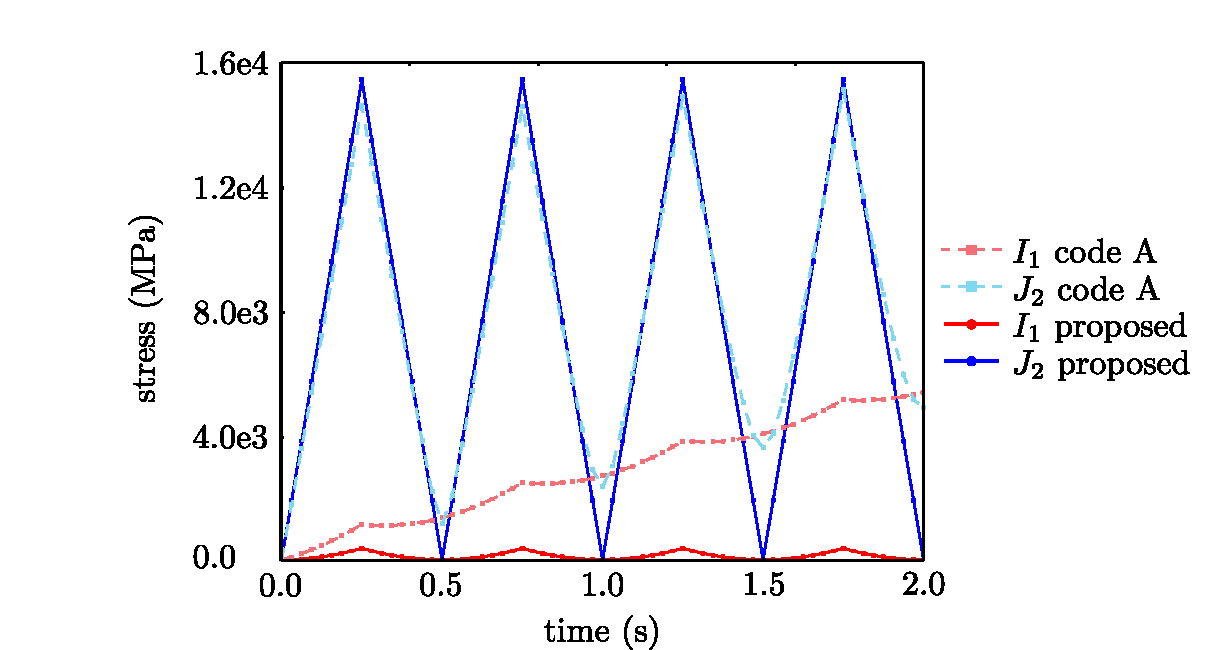
\includegraphics[scale=0.75]{media/twisted_prism.pdf}
% where an .eps filename suffix will be assumed under latex,
% and a .pdf suffix will be assumed for pdflatex
\caption{Stress measures plotted vs. time for the twisting prism problem, where $I_1$ is the first invariant of the Cauchy stress tensor, and $J_2$ is the second invariant of the deviatoric stress tensor}
\label{fig.twisted_prism-cm1}
\end{figure}
\negparafig

%%%%%%%%%%%%%%%%%%%%%%%%%%%%%%%%%%%%%%%%%%%%%%%
%%%%%%%%%%%%%%%%%%%%%%%%%%%%%%%%%%%%%%%%%%%%%%%
\section{Performance Evaluation of Nonlinear Solution Convergence}
%

\begin{figure}[!tbhp]
\centering
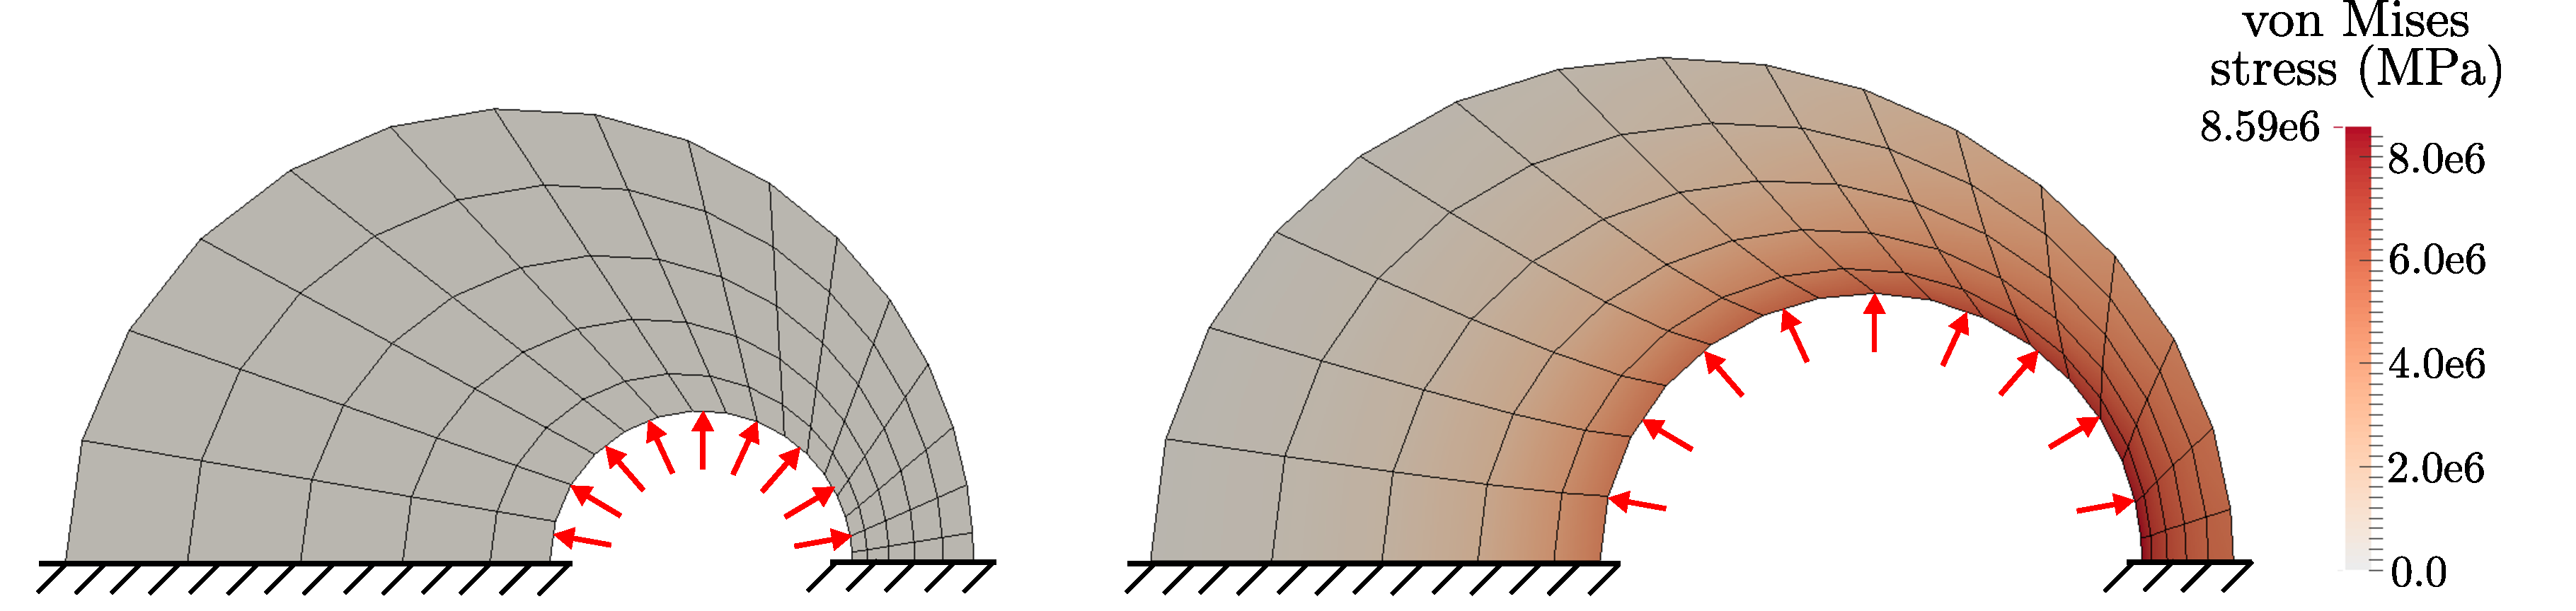
\includegraphics[scale=0.28]{media/ring_problem}
% where an .eps filename suffix will be assumed under latex,
% and a .pdf suffix will be assumed for pdflatex
\caption{Pressurized eccentric cylinder modeled with half-symmetry.}
\label{fig.ring}
\end{figure}

\begin{table}[]
\centering
\caption{Number of Newton-Raphson iterations per time step for the eccentric cylinder problem}
\label{tab.ring}
\begin{tabular}{|c|c|c|c|}
\hline
Step & Hughes-Winget & Rashid (1993) & Proposed Algorithm  \\ \hline
1  & 3 & 3  & 3 \\ \hline
2  & 2 & 2  & 2 \\ \hline
3  & 2 & 2  & 2 \\ \hline
4  & 2 & 2  & 2 \\ \hline
5  & 2 & 2  & 2 \\ \hline
6  & 2 & 3  & 2 \\ \hline
7  & 2 & 3  & 2 \\ \hline
8  & 2 & 3  & 2 \\ \hline
9  & 3 & 4  & 3 \\ \hline
10 & 4 & 27 & 4\\ \hline
\end{tabular}
\end{table}

\begin{table}[]
\centering
\caption{Number of Newton-Raphson iterations using an inconsistent linearization}
\label{tab.ring_tangents}
\begin{tabular}{|c|c|c|c|c|}
\hline
Step & Consistent & Rotation Off & Pressure Off & Rotation \& Pressure Off \\ \hline
1  & 3 & 5   & 6  & 6 \\ \hline
2  & 2 & 5   & 7  & 8 \\ \hline
3  & 2 & 6   & 9  & 10 \\ \hline
4  & 2 & 6   & 11 & 13 \\ \hline
5  & 2 & 8   & 14 & 16 \\ \hline
6  & 2 & 10  & 18 & 20 \\ \hline
7  & 2 & 14  & 25 & 24 \\ \hline
8  & 2 & 22  & 42 & 31 \\ \hline
9  & 3 & 40  & 123 & 41 \\ \hline
10 & 4 & 771 & $>$1000 & 784 \\ \hline
\end{tabular}
\end{table}
\section{Conclusions}
%
\section{Appendix}
%


%%%%%%%%%%%%%%%%%%%%%%%%%%%%%%%%%%%%%%%%%%%%%%%%%%%%%%%%%%%%%%%%%%%%%%%%

\bibliography{references}

%%%%%%%%%%%%%%%%%%%%%%%%%%%%%%%%%%%%%%%%%%%%%%%%%%%%%%%%%%%%%%%%%%%%%%%%

\end{document}